This appendix presents the details of the theoretical framework.

\begin{proof}[Proof of Proposition \ref{chap3-prp:converge}]
    The value converges as $\lim_{t\to+\infty} a_t = a^\star$ since $(\eta_a,\phi_a)\in(\mathbb{R}^\star_{+})^2$. The rate of convergence $\eta_a/(\eta_a+\phi_a)$ is a decreasing in $\phi_a/\eta_a$. The smaller the rate of convergence, the faster the speed of convergence. Therefore, the speed of convergence is an increasing function of the relative weight of the group consistency with respect to the time consistency in the utility function.
\end{proof}

\begin{proof}[Proof of Proposition \ref{chap3-prp:shock}]
$\forall s_t\in\{\underline{s}, \overline{s}\}, \forall a_t\in\mathbb{R},~\exists \Delta{a_t} > \Delta\widetilde{a}_t$ such that $\lim_{t\to+\infty} a_{t+1} = a^\star(-s_t)$
\end{proof}

\begin{proof}[Proof of Proposition \ref{chap3-prp:relevant}]
Starting with the expression of the indifference value $\widetilde{a}$ from equation, it is straightforward to show that $\frac{\partial^2\widetilde{a}}{\partial(\overline{b}-\underline{b})^2}>0$. In this example, $\widetilde{a}$ is a convex function of $\overline{b}-\underline{b}$. Thus, the greater the gap between both groups in value $b$ with respect to value $a$, the greater the information shock in value $a$ has to be so that the agent identifies to the other group. Therefore, the less relevant is this latter value in its choice of group membership.
\end{proof}

\begin{proof}[Proof of Proposition \ref{chap3-prp:spillover}]
If $\overline{b}-\underline{b}\neq 0$, then $\exists \Delta{a_t}$ such that $a_{t-1}^\prime > \widetilde{a}_{t-1}$ which implies that the individual identifies to the other group in period $t$. Therefore, both values $a_t$ and $b_t$ change.
\end{proof}

\textbf{Theoretical framework with three groups.}
One may ask to which extent the results hold with more than two groups. So, suppose that instead of having two groups in the reference population, we introduce a third group between both groups. I refer to the former groups as $s_A$ and $s_C$ instead of $\overline{s}$ and $\underline{s}$, while $s_B$ is the new group.

Starting with the single-value model, the ranking is as follows $a_A < a_B < a_C$. Reproducing figure \ref{chap3-fig:theory-choice-a} but with three groups leads to figure \ref{chap3-fig:theory-choice3-a}.
\begin{figure}[!ht]
    \centering
    \caption{Indifference value and group membership (with three groups)}
    \label{chap3-fig:theory-choice3-a}
    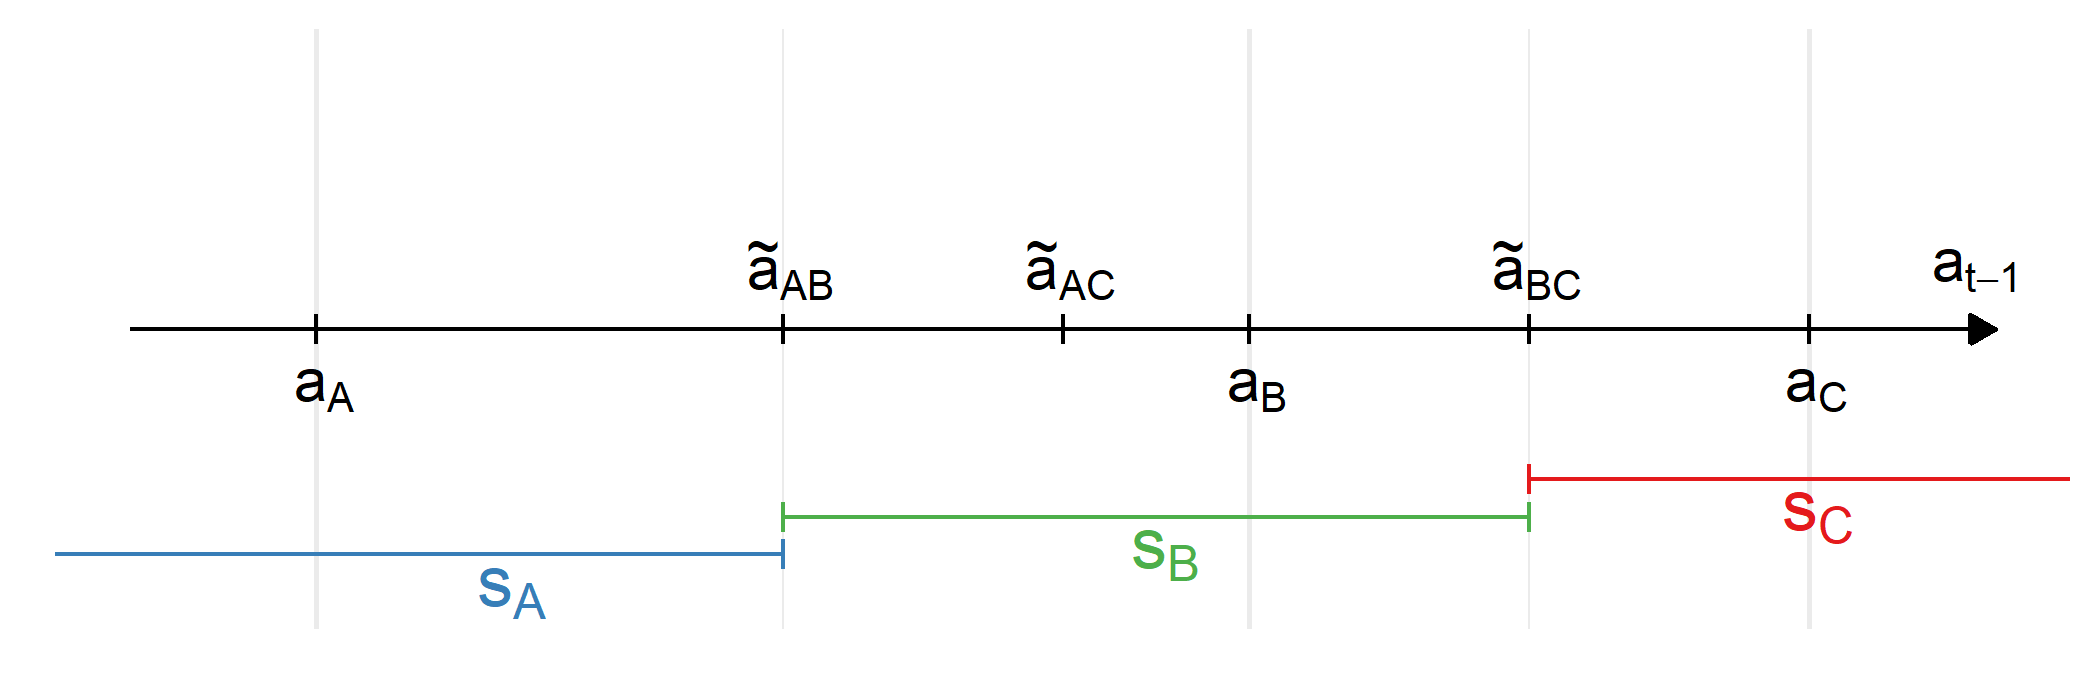
\includegraphics[width=.8\linewidth]{chap3/graphic/theory-choice3-a.png}
	\vspace{-3em}
	\justify\singlespacing\footnotesize{\textit{Notes:} This figure is an extension of figure \ref{chap3-fig:theory-choice-a} when there are three groups instead of two in the single value model. The figure presents the indifference values $\widetilde{a}_{ij}$ which are defined as the threshold values $a$ in $t-1$ such that the agent is indifferent between two groups. When the value $a$ in previous period lie in the area of one group, the agent prefers to identify to this group.}
\end{figure}
Introducing an additional group does not change the indifference value between two groups---which remains the midpoint value.
Propositions \ref{chap3-prp:converge} and \ref{chap3-prp:shock} hold in the three-group model.

Consider the two-value model by introducing the second value $b$. Assume the following ranking $a_C < a_B < a_A$ and $b_C < b_B < b_A$, which means that values are positively correlated across groups. I use the simplest case as an example, but other types of ranking are possible. Suppose the setup of section \ref{chap3-theoretical} with respect to the agent. She belongs to the group with the lowest value $a$, hence, $s_A$. It is still possible to derive the expression of the indifference value between the groups $A$ and $j\in\{B,C\}$ from equation \eqref{chap3-eq:indiff}, namely,
\begin{equation}\label{chap3-eq:indiff2}
    \widetilde{a}_{Aj} = \widehat{a}_{Aj} + \frac{1}{2\gamma}\frac{\big(b_j-b_A\big)^2}{a_j-a_A},
\end{equation}
where $\widehat{a}_{Aj}$ is the midpoint value between those of both groups $A$ and $j$. Since $a_j-a_A > 0$, it means that the second term of \eqref{chap3-eq:indiff2} is positive. As a result, the indifference value $\widetilde{a}$ is greater than the midpoint value. Both frontiers are pushed further right with respect to the single-value model in figure \ref{chap3-fig:theory-choice3-a}.

Under those conditions, it is still always possible to find an information shock such that the agent changes her group. Therefore, both propositions \ref{chap3-prp:relevant} and \ref{chap3-prp:spillover} hold. Although spillover effects still exist, their magnitudes are different with respect to the case with the two groups. Information shocks that move $a^\prime_{t-1}$ between $\widetilde{a}_{AB}$ and $\widetilde{a}_{BC}$ generate smaller spillover effects---with respect to the two-group model---as the agent identifies to the group $s_B$; while shocks that move $a^\prime_{t-1}$ beyond $\widetilde{a}_{BC}$ generate larger spillover effects.